
%\vspace{-0.5em}
\section{Introduction}
\label{sec:intro}

\begin{figure}[t!]
    \centering
    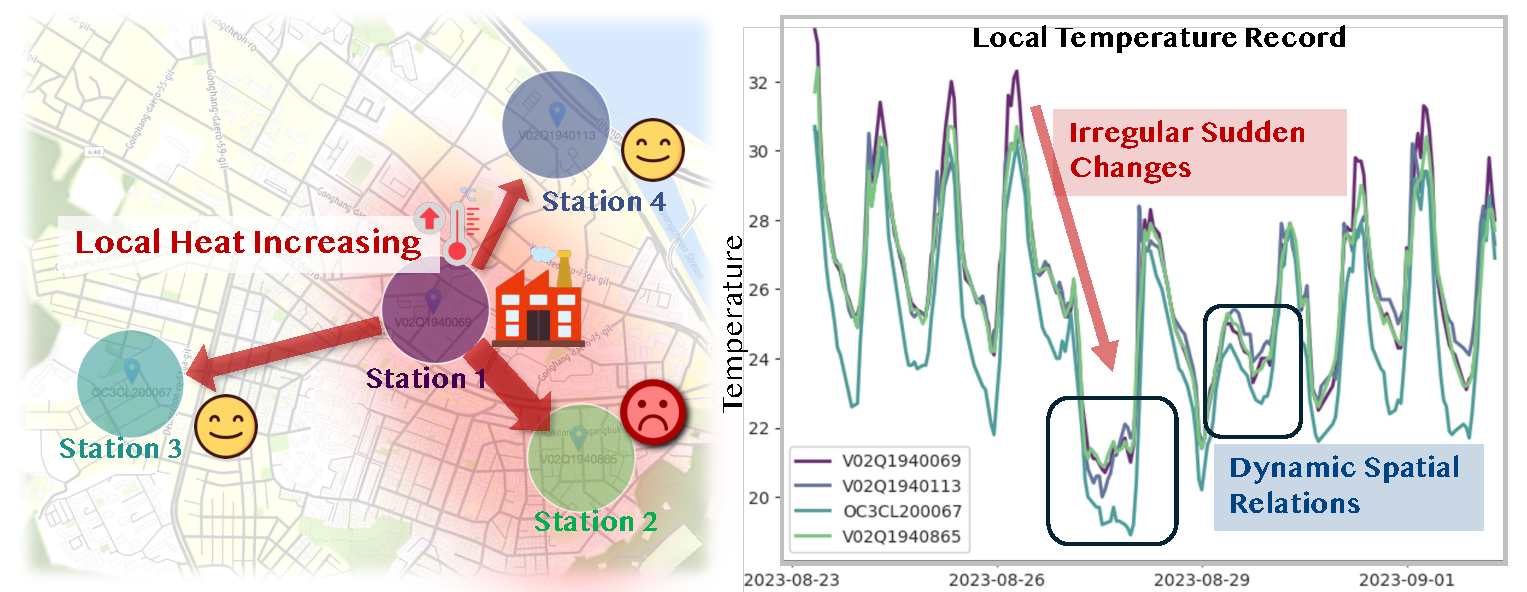
\includegraphics[width=1.0\linewidth]{resources/intro_1.pdf}
    \vspace{-1em}
    \caption{Introduction of Urban Heat Island effect. \textit{Left:}  Regional UHI effects are closely linked to the regional environment. \textit{Right:} Urban thermodynamics is temporal irregular and has highly dynamic spatial relations.}
    \label{fig:intro_data}
    \vspace{-1.5em}
\end{figure}

Rapid urbanization has caused a host of environmental and sustainability challenges in cities and beyond~\cite{krupat1985people,keivani2009review,zheng2014urban,wen2023diffstg,zou2024learning,zou2025deep}. Within cities, the dynamic interaction between natural elements and human activities leads to localized heat accumulation, thereby giving rise to the sophisticated \textbf{Urban Heat Island (UHI)} effect~\cite{lyu2022integrated,yoo2018investigating,li2019urban}. 
Recognizing the critical importance of this issue, the United Nations has identified "\textit{cities and human settlements climate resilient and sustainable}" as a key sustainable development goal~\cite{lu2015policy}. This mandate, coupled with the challenges posed by global warming ~\cite{alcoforado2008global,santamouris2014energy,santamouris2015impact} and the increasing vulnerability of elderly and at-risk populations~\cite{zhu2023urban,park2021differing,heaviside2017urban}, underscores the urgent need to develop robust thermodynamic models for accurate UHI forecasting.


Forecasting the UHI effect, usually quantified through urban field temperatures, presents distinct challenges compared to conventional climate forecasting. Most existing studies have predominantly utilized macro-scale and qualitative approaches, either by contrasting temperatures between urban cores and their surrounding suburban areas~\cite{rizwan2008review,yang2016research,tehrani2024predicting} or by interpolating land temperatures using remote sensing observations~\cite{mirzaei2010approaches,peng2012surface,diem2024remote,zhou2018satellite}. However, both the UHI effect and the associated field temperature demonstrate remarkable variability within urban areas, exhibiting gradients that reflect differing levels of urban development~\cite{lyu2022integrated,yoo2018investigating}. Neighborhood-specific factors, such as the presence of green spaces, water bodies, and land function, further contribute to this spatial heterogeneity. Consequently, the inherent complexity of these urban thermodynamics renders coarse-grained remote sensing data and traditional numerical inference methods~\cite{adilkhanova2022recent,yang2022quantitative} insufficient for this application.

Recently, data-driven methods such as GenCast~\cite{price2025probabilistic} and Pangu-weather~\cite{bi2022pangu,xu2024improvement} have shown impressive accuracy in climate forecasting by modeling global atmospheric dynamics. However, when addressing regional climate phenomena at low altitudes, they tend to underperform compared to traditional numerical models~\cite{olivetti2024data,huang2025initial}. This discrepancy reveals the significant challenge of modeling urban thermodynamics for fine-grained UHI effect forecasting. As shown in Figure \ref{fig:intro_data}, firstly, UHI patterns are closely intertwined with various environmental factors, leading to complex spatial heterogeneity that further complicates modeling effects. Secondly, fine-grained regional temperature variations are more sensitive and irregular than those found in general atmospheric circulation~\cite{price2023gencast,nguyen2023scaling} or in other spatio-temporal phenomena such as regional traffic flow~\cite{liang2023airformer,yin2021deep,li2023dynamic}.  As a result, key challenges remain in effectively capturing spatio-temporal thermodynamics of local thermal systems and integrating essential environmental information without introducing noise.

\begin{figure}[t!]
    \centering
    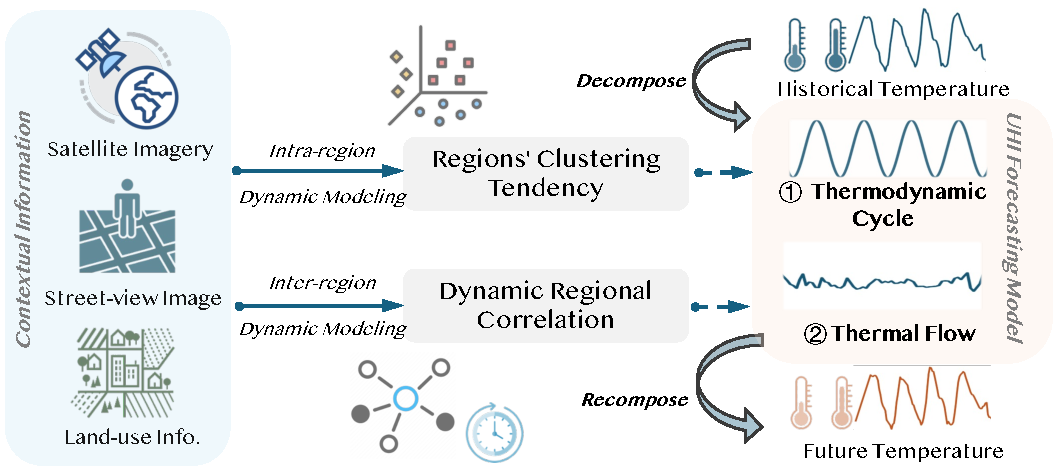
\includegraphics[width=1\linewidth]{resources/intro_2.pdf}
    \vspace{-1em}
    \caption{Insight of the framework.}
    \label{fig:intro_method}
    \vspace{-1.5em}
\end{figure}
In theory, the problem can be addressed using the heat equation by treating spatio-temporal thermodynamics as a flow physics problem. Accurate modeling of local thermodynamics becomes promising by incorporating urban environmental information as boundary conditions for the nonlinear partial differential heat equation~\cite{widder1976heat,doob1955probability,lewis2004fundamentals}, although an analytical solution for such an equation is not achievable. In this paper, guided by this equation, we introduce \model, a data-driven framework for modeling local thermodynamics with contextual information. To enable data-driven instantiation of the partial differential equation, local thermodynamics are decomposed into intra-region \textbf{thermodynamic cycles}~\cite{chen2010review,qian2015thermodynamics} and inter-region \textbf{thermal flows}~\cite{lewis2004fundamentals,zienkiewicz1981general} (see Fig. \ref{fig:intro_method}).

\begin{figure*}
    \centering
    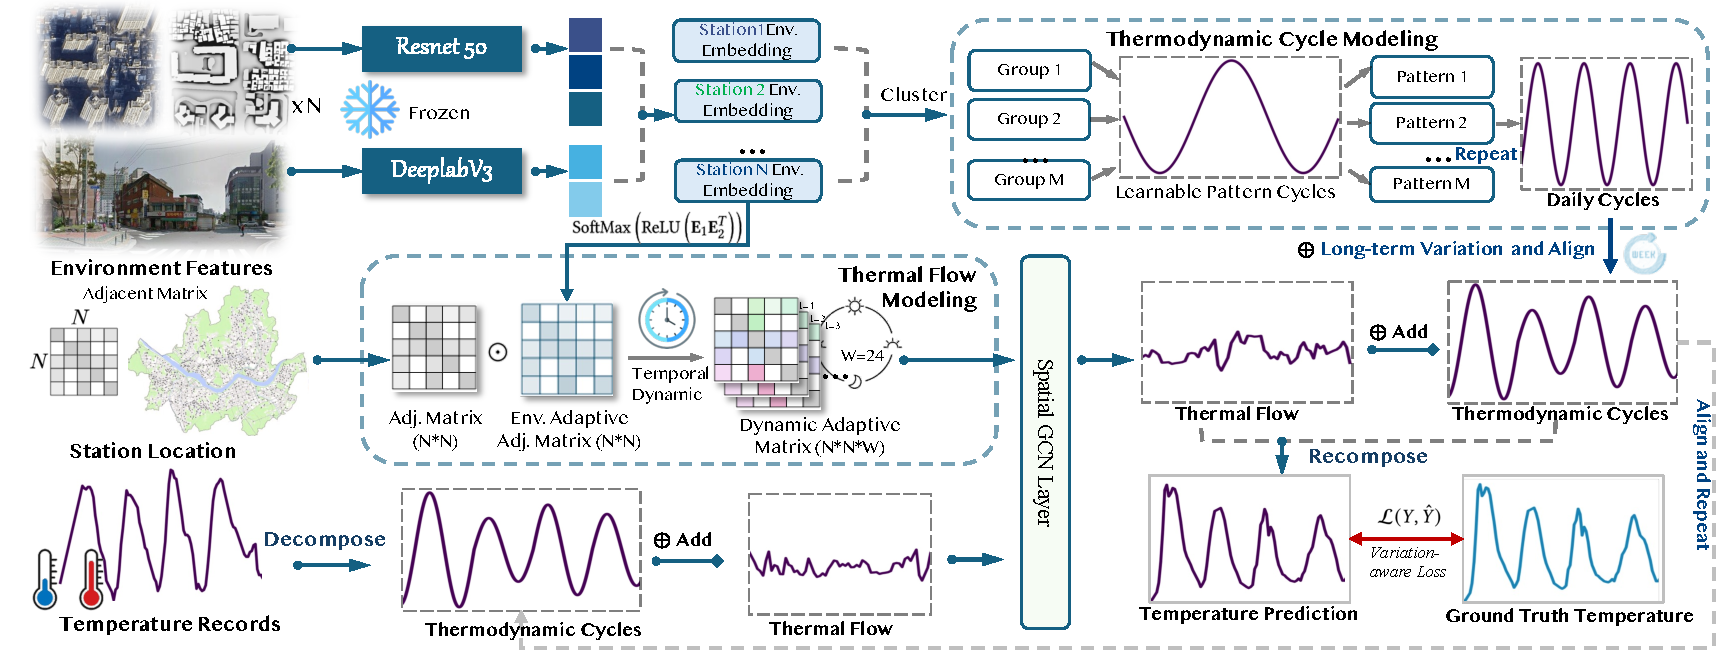
\includegraphics[width=0.95\linewidth]{resources/framework.pdf}
    \vspace{-0.5em}
    \caption{An illustration of our proposed \model framework.}
    \vspace{-1em}
    \label{fig:frame}
\end{figure*}
Firstly, according to thermal equation, without disturbance, the daily thermal cycle of a region is stable and distinct, referred to as the intra-region \textbf{thermodynamic cycle}. This cycle contributes to the daily temperature variations and is determined by the region's Specific Heat Capacity (SHC), which is influenced by the components of the surrounding environment. Inspired by these characteristics, we cluster stations into groups based on their similar environmental features and design a temporal periodicity learning block to explicitly instantiate the different temporal cycles. This approach efficiently models the regional thermodynamic cycle while avoiding complex over-fitting.

Secondly, inter-region \textbf{thermal flow} refers to the thermal transfer process of local heat variation between adjacent regions caused by temperature differences, contributing to irregular temporal variations in temperature. Although these mechanics can be naturally represented through spatial graph convolution~\cite{zou2024learning,song2020spatial,lu2020spatiotemporal,alet2019graph,sanchez2020learning}, heat transfer in regional thermal equation is anisotropic in different directions and times due to various environment situations. This behavior goes beyond the capacity of a vanilla distance-based adjacency matrix. Therefore, we introduce a dynamic adaptive convolution block to instantiate the anisotropic thermal flow. Specifically, we introduce a context-aware adaptive graph convolution to learn the spatial anisotropy from environment features. For the temporal anisotropy, we design lightweight temporal dynamic learning mechanics to represent the temporal variation of heat transfer without introducing redundant model complexity.

Modeling the two thermal mechanics separately provides clear solutions. However, orderly recomposing them for UHI effect forecasting presents another challenge in terms of an imbalanced value range. The temperature temporal fluctuations caused by local thermal flow are minor compared to the daily thermal cycle, which may lead to these fluctuations being misinterpreted as noise by the cycle learning block, and vice versa. While explicitly modeling the daily cycle in our temporal learning block can help mitigate this issue, the training process remains unstable. To address this challenge, we introduce a fluctuation fine-tuning training strategy and a variation-aware loss function within our framework to effectively support our decomposition strategy.

Furthermore, we conduct an in-depth study to demonstrate the necessity and effectiveness of our framework in the context of fine-grain temperature predictions and warnings for extreme heat events. In addition, we deploy it on our SeoUHI platform to deliver real-world UHI effect forecasting and notifications to the citizens in the Seoul area. Our contributions are summarized as follows:




(1) We propose \textit{DeepUHI}, the first data-driven context-aware framework for modeling local thermodynamics based on the heat equation. In our methodology, we introduce an explainable heat decomposition framework to represent thermodynamics from the perspectives of \textit{thermodynamic cycles} and \textit{thermal flows}, which systematically and concisely incorporates urban environmental data into the forecasting process.

(2) We conduct extensive experiments to demonstrate the necessity and effectiveness of our proposed framework. Comprehensive results indicate that it outperforms existing time-series and spatio-temporal forecasting baselines in UHI effect forecasting and warning tasks while maintaining high computational efficiency.

(3) We collect and introduce \textit{SeoulTemp}, the first fine-grained urban temperature dataset that includes field environment data across multiple modalities. This dataset encompasses a total of 947 temperature stations covering 605 $km^{2}$ of land in Seoul from 2021 to 2024, specifically targeting spatio-temporal UHI effect forecasting at the street level in urban areas.

(4) Our framework and model are deployed on the SeoUHI platform, providing precise short-term (day-ahead) UHI effect and extreme temperature notification services for over 10 million citizens in the Seoul area.




% In this work, we first introduce a real-word dataset, called \textit{SeoulTemp}, the first fine-grained, publicly available, and multi-modal dataset specifically targeting spatio-temporal UHI effect predictions for the Seoul area at the street level. As shown in Figure 1,
% the \textit{SeoulTemp} dataset is composed of three modalities of data, i.e.,
% Satellite Imagery, Street-view Imagery, Seoul Land-use Dataset, SDot Temperature Database, covering a total of 947 temperature stations within 605 $km^{2}$ land of Seoul from 2021 to 2024. The satellite and street-view imagery comprehensively describe the environment around each station. The Seoul Land-use Dataset, obtained from the Korea EGIS, offers fine-grain land-use information for each station. The SDot Temperature Dataset, sourced
% from the Seoul SDot project, contains hourly field average temperature of stations.